% Options for packages loaded elsewhere
\PassOptionsToPackage{unicode}{hyperref}
\PassOptionsToPackage{hyphens}{url}
%
\documentclass[
]{article}
\usepackage{amsmath,amssymb}
\usepackage{iftex}
\ifPDFTeX
  \usepackage[T1]{fontenc}
  \usepackage[utf8]{inputenc}
  \usepackage{textcomp} % provide euro and other symbols
\else % if luatex or xetex
  \usepackage{unicode-math} % this also loads fontspec
  \defaultfontfeatures{Scale=MatchLowercase}
  \defaultfontfeatures[\rmfamily]{Ligatures=TeX,Scale=1}
\fi
\usepackage{lmodern}
\ifPDFTeX\else
  % xetex/luatex font selection
\fi
% Use upquote if available, for straight quotes in verbatim environments
\IfFileExists{upquote.sty}{\usepackage{upquote}}{}
\IfFileExists{microtype.sty}{% use microtype if available
  \usepackage[]{microtype}
  \UseMicrotypeSet[protrusion]{basicmath} % disable protrusion for tt fonts
}{}
\makeatletter
\@ifundefined{KOMAClassName}{% if non-KOMA class
  \IfFileExists{parskip.sty}{%
    \usepackage{parskip}
  }{% else
    \setlength{\parindent}{0pt}
    \setlength{\parskip}{6pt plus 2pt minus 1pt}}
}{% if KOMA class
  \KOMAoptions{parskip=half}}
\makeatother
\usepackage{xcolor}
\usepackage[margin=1in]{geometry}
\usepackage{longtable,booktabs,array}
\usepackage{calc} % for calculating minipage widths
% Correct order of tables after \paragraph or \subparagraph
\usepackage{etoolbox}
\makeatletter
\patchcmd\longtable{\par}{\if@noskipsec\mbox{}\fi\par}{}{}
\makeatother
% Allow footnotes in longtable head/foot
\IfFileExists{footnotehyper.sty}{\usepackage{footnotehyper}}{\usepackage{footnote}}
\makesavenoteenv{longtable}
\usepackage{graphicx}
\makeatletter
\def\maxwidth{\ifdim\Gin@nat@width>\linewidth\linewidth\else\Gin@nat@width\fi}
\def\maxheight{\ifdim\Gin@nat@height>\textheight\textheight\else\Gin@nat@height\fi}
\makeatother
% Scale images if necessary, so that they will not overflow the page
% margins by default, and it is still possible to overwrite the defaults
% using explicit options in \includegraphics[width, height, ...]{}
\setkeys{Gin}{width=\maxwidth,height=\maxheight,keepaspectratio}
% Set default figure placement to htbp
\makeatletter
\def\fps@figure{htbp}
\makeatother
\setlength{\emergencystretch}{3em} % prevent overfull lines
\providecommand{\tightlist}{%
  \setlength{\itemsep}{0pt}\setlength{\parskip}{0pt}}
\setcounter{secnumdepth}{-\maxdimen} % remove section numbering
\ifLuaTeX
  \usepackage{selnolig}  % disable illegal ligatures
\fi
\usepackage{bookmark}
\IfFileExists{xurl.sty}{\usepackage{xurl}}{} % add URL line breaks if available
\urlstyle{same}
\hypersetup{
  pdftitle={Tunnel diode 2024},
  pdfauthor={YDS},
  hidelinks,
  pdfcreator={LaTeX via pandoc}}

\title{Tunnel diode 2024}
\author{YDS}
\date{2024-06-10}

\begin{document}
\maketitle

\section{Введение}\label{ux432ux432ux435ux434ux435ux43dux438ux435}

Туннельные диоды были открыты учёным Эсаки и используют эффект
квантового туннелирования электронов через потенциальный барьер.

Этот эффект связан с волновой природой электронов, благодаря которой они
могут попадать в классически запрещённые области.

Существует несколько видов туннельных диодов. Наиболее типичные сделаны
на основе PN-переходов (рис. 1), но есть и другие (например,
резонансно-туннельные диоды, диоды на основе свехрешёток и т.д.)

\begin{figure}
\centering
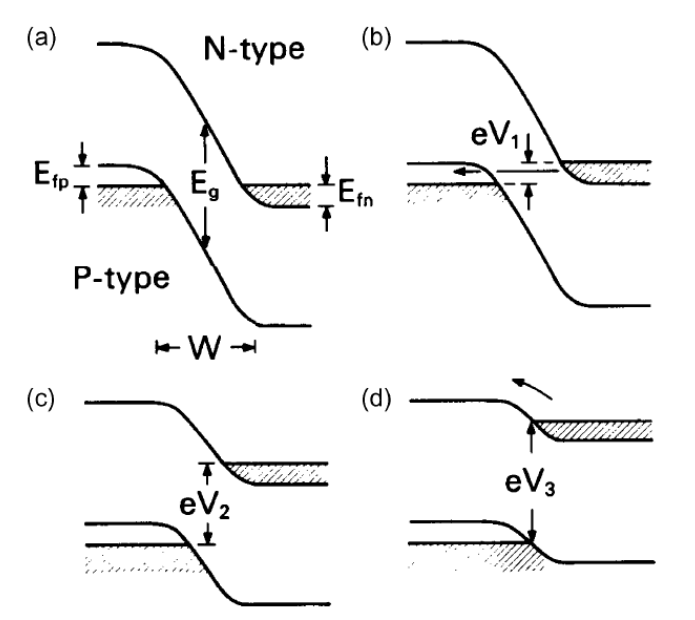
\includegraphics[width=4.16667in,height=\textheight]{images/esaki.png}
\caption{Рисунок 1. Схема туннельного диода Эсаки {[}1{]}.}
\end{figure}

\[ \]

Туннельные диоды известны тем, что на их ВАХ наблюдается область
отрицательного дифференциального сопротивления (отрицательной
дифференциальной проводимости --- ОДП). Дифференциальная проводимость
определяется как:

\[ \Omega_{d}=\frac{dI}{dV} \] Обычная проводимость --- отношение тока к
напряжению --- не может быть отрицательной, а дифференциальная может.
При этом ток положительный, но начинает падать при росте напряжения. Это
можно видеть на рис. 2.

\begin{figure}
\centering
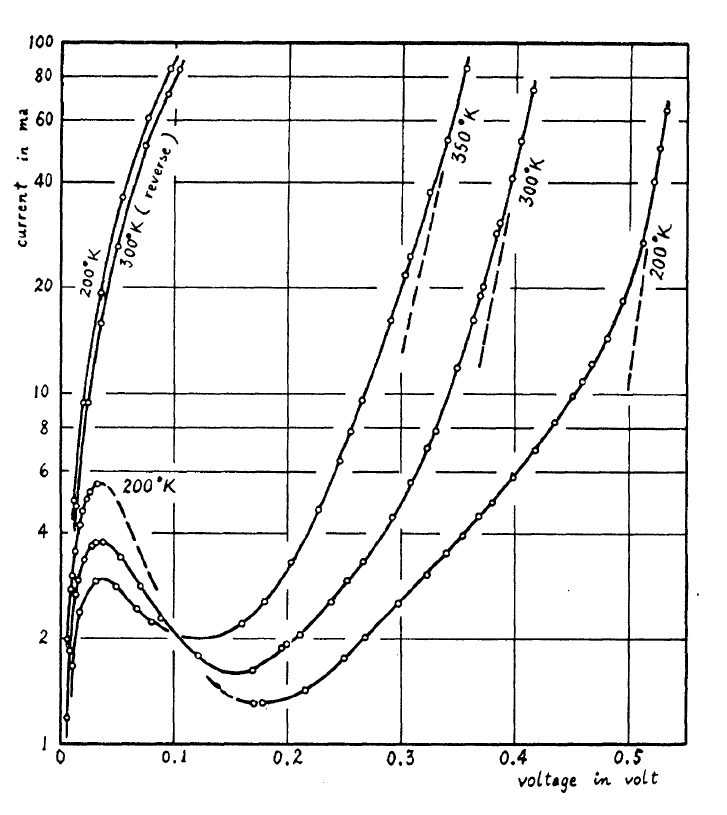
\includegraphics[width=3.125in,height=\textheight]{images/iv-curve.png}
\caption{Рисунок 2. ВАХ туннельного диода {[}1{]}.}
\end{figure}

\[ \]

Участок ОДП может быть использован для генераторов переменного тока
(генераторов колебаний), потому что он позволяет компенсировать
внутреннее сопротивление цепи и избежать затухания колебаний.

\section{Обзор
литературы}\label{ux43eux431ux437ux43eux440-ux43bux438ux442ux435ux440ux430ux442ux443ux440ux44b}

Ток через туннельный диод можно рассчитать по формуле Эсаки {[}2{]}.

\[I(V)=\frac{em_{e}kT}{2\pi^{2}\hbar^{3}}\int_{0}^{\infty}T_{c}\left(E_{\perp}\right)\left[\ln\left(1+\exp\frac{E_{Fn}+eV-E_{\perp}}{kT}\right)-\ln\left(1+\exp\frac{E_{Fp}-E_{\perp}}{kT}\right)\right]\mathrm{d}E_{\perp} \tag{1}\]

Где \(T_c\) --- вероятность (коэффициент) прохождения электронов через
барьер, \(E_{\perp}\) --- кинетическая энергия электронов в направлении
границы между P и N областями, которая отсчитывается от дна зоны
проводимости \(E_c\).

Логарифмы описывают распределение электронов по энергиям в P и N
областях.

Для работы туннельного диода области N и P должны быть сильно
легированы, то там должно быть очень много примесей. Тогда при \(V=0\)
уровни Ферми будут находится внутри зоны проводимости в N области и
внутри валентной зоны в P области, как изображено на рис. 3а.

\begin{figure}
\centering
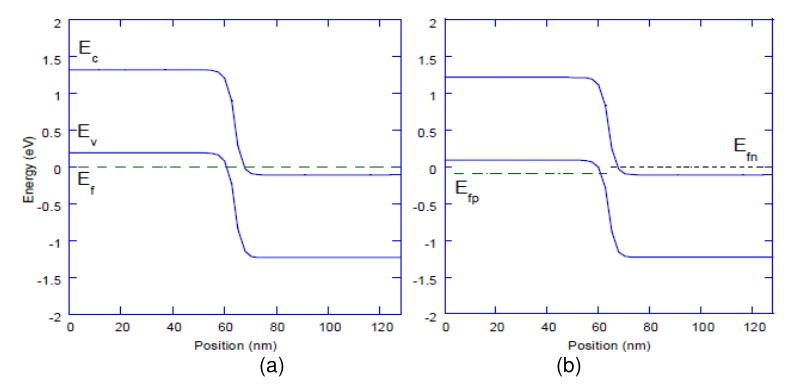
\includegraphics[width=5.20833in,height=\textheight]{images/diode-scheme-2.png}
\caption{Рисунок 3. Зонная структура туннельного диода при а) \(V=0\) и
b) \(V>0\) {[}3{]}.}
\end{figure}

\[ \]

Вероятность прохождения барьера может быть рассчитана с помощью
квантовой механики для барьеров любой формы. В данном случае барьер
похож на треугольный (рис. 4), но можно его считать и прямоугольным. При
повышении напряжения уровни Ферми будут смещаться друг относительно
друга и барьер между P и N областями будет уменьшаться (рис. 3b).

\begin{figure}
\centering
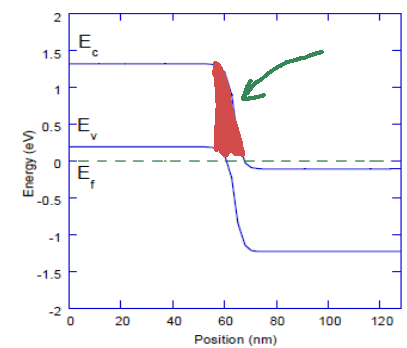
\includegraphics[width=2.60417in,height=\textheight]{images/diode-scheme-3.png}
\caption{Рисунок 4. Энергетический барьер.}
\end{figure}

\[ \]

Самый простой вид имеет коэффициент прохождения для очень узкого барьера
в виде дельта-функции:

\[U(x)=\alpha \delta(x),\qquad \alpha = Ha \tag{2}\]

где \(H\) --- высота барьера в единицах энергии (эВ), а \(a\) --- ширина
барьера (например, в нм).

Для неё вероятность прохождения имеет вид:

\[T_c(E)=\frac{E}{E+\frac{m_e \alpha^2}{2\hbar^2}} \tag{3}\]

\section{Основные
формулы}\label{ux43eux441ux43dux43eux432ux43dux44bux435-ux444ux43eux440ux43cux443ux43bux44b}

\subsection{Константы}\label{ux43aux43eux43dux441ux442ux430ux43dux442ux44b}

\begin{longtable}[]{@{}
  >{\centering\arraybackslash}p{(\columnwidth - 8\tabcolsep) * \real{0.2000}}
  >{\centering\arraybackslash}p{(\columnwidth - 8\tabcolsep) * \real{0.2000}}
  >{\centering\arraybackslash}p{(\columnwidth - 8\tabcolsep) * \real{0.2000}}
  >{\centering\arraybackslash}p{(\columnwidth - 8\tabcolsep) * \real{0.2000}}
  >{\centering\arraybackslash}p{(\columnwidth - 8\tabcolsep) * \real{0.2000}}@{}}
\toprule\noalign{}
\begin{minipage}[b]{\linewidth}\centering
Обозначение
\end{minipage} & \begin{minipage}[b]{\linewidth}\centering
Формула
\end{minipage} & \begin{minipage}[b]{\linewidth}\centering
Переменная
\end{minipage} & \begin{minipage}[b]{\linewidth}\centering
Значение
\end{minipage} & \begin{minipage}[b]{\linewidth}\centering
Единицы
\end{minipage} \\
\midrule\noalign{}
\endhead
\bottomrule\noalign{}
\endlastfoot
\(k\) & \(k\) & k\_boltzmann & 8.62e-5 & эВ\(\cdot\)K\(^{-1}\) \\
\(q\) & \(\displaystyle \frac{e}{\hbar}\) & e\_h & 2.43e-4 &
А\(\cdot\)эВ\(^{-1}\) \\
\(K\) & \(\displaystyle \frac{\hbar^2}{m_0}\) & h2\_m0 & 0.0762 &
эВ\(\cdot\)нм\(^2\) \\
\(C\) & \(\displaystyle \frac{e^2}{4\pi \varepsilon_0}\) & e2\_4pieps0 &
1.44 & эВ\(\cdot\)нм \\
\end{longtable}

\subsection{Исходные
параметры}\label{ux438ux441ux445ux43eux434ux43dux44bux435-ux43fux430ux440ux430ux43cux435ux442ux440ux44b}

\begin{longtable}[]{@{}
  >{\centering\arraybackslash}p{(\columnwidth - 10\tabcolsep) * \real{0.1667}}
  >{\centering\arraybackslash}p{(\columnwidth - 10\tabcolsep) * \real{0.1667}}
  >{\centering\arraybackslash}p{(\columnwidth - 10\tabcolsep) * \real{0.1667}}
  >{\centering\arraybackslash}p{(\columnwidth - 10\tabcolsep) * \real{0.1667}}
  >{\centering\arraybackslash}p{(\columnwidth - 10\tabcolsep) * \real{0.1667}}
  >{\centering\arraybackslash}p{(\columnwidth - 10\tabcolsep) * \real{0.1667}}@{}}
\toprule\noalign{}
\begin{minipage}[b]{\linewidth}\centering
Величина
\end{minipage} & \begin{minipage}[b]{\linewidth}\centering
Обозначение
\end{minipage} & \begin{minipage}[b]{\linewidth}\centering
Переменная
\end{minipage} & \begin{minipage}[b]{\linewidth}\centering
Диапазон
\end{minipage} & \begin{minipage}[b]{\linewidth}\centering
Значение
\end{minipage} & \begin{minipage}[b]{\linewidth}\centering
Единицы
\end{minipage} \\
\midrule\noalign{}
\endhead
\bottomrule\noalign{}
\endlastfoot
Ширина запр. зоны & \(E_g\) & band\_gap & 0.2 -- 2 & 1.12 & эВ \\
Эфф. масса эл. & \(m_e\) & eff\_mass\_e & 0.01 -- 1 & 0.19 & \(m_0\) \\
Эфф. масса дыр. & \(m_h\) & eff\_mass\_h & 0.01 -- 1 & 0.49 & \(m_0\) \\
Диэлектр. прониц. & \(\varepsilon\) & dielectric & 1 -- 15 & 11.7 & - \\
Температура & \(T\) & temperature & 4 -- 400 & 300 & К \\
Конц. доноров & \(N_d\) & donor\_conc & 1e-4 -- 0.1 & 0.1 &
нм\(^{-3}\) \\
Конц. акцепторов & \(N_a\) & accept\_conc & 1e-4 -- 0.1 & 0.1 &
нм\(^{-3}\) \\
\end{longtable}

\subsection{Вторичные
параметры}\label{ux432ux442ux43eux440ux438ux447ux43dux44bux435-ux43fux430ux440ux430ux43cux435ux442ux440ux44b}

\begin{longtable}[]{@{}
  >{\centering\arraybackslash}p{(\columnwidth - 6\tabcolsep) * \real{0.2500}}
  >{\centering\arraybackslash}p{(\columnwidth - 6\tabcolsep) * \real{0.2500}}
  >{\centering\arraybackslash}p{(\columnwidth - 6\tabcolsep) * \real{0.2500}}
  >{\centering\arraybackslash}p{(\columnwidth - 6\tabcolsep) * \real{0.2500}}@{}}
\toprule\noalign{}
\begin{minipage}[b]{\linewidth}\centering
Обозначение
\end{minipage} & \begin{minipage}[b]{\linewidth}\centering
Формула
\end{minipage} & \begin{minipage}[b]{\linewidth}\centering
Переменная
\end{minipage} & \begin{minipage}[b]{\linewidth}\centering
Единицы
\end{minipage} \\
\midrule\noalign{}
\endhead
\bottomrule\noalign{}
\endlastfoot
\(N_c\) &
\(\displaystyle 2 \cdot \left( \frac{m_e kT}{2\pi K} \right)^{3/2}\) &
n\_c & нм\(^{-3}\) \\
\(N_v\) &
\(\displaystyle 2 \cdot \left( \frac{m_h kT}{2\pi K} \right)^{3/2}\) &
n\_v & нм\(^{-3}\) \\
\(E_{Fn}-E_c\) & \(\displaystyle kT \ln \left( \frac{N_d}{N_c} \right)\)
& fermi\_n & эВ \\
\(E_{Fp}-E_v\) & \(\displaystyle kT \ln \left( \frac{N_v}{N_a} \right)\)
& fermi\_p & эВ \\
\(\Delta \Phi\) &
\(\displaystyle E_{Fn} - E_c -\left(E_{Fp} - E_v \right) +E_g\) &
delta\_phi & эВ \\
\(W^3\) &
\(\displaystyle \frac{\pi C K k T}{m_e} \frac{N_a N_d}{N_a+N_d}\) &
transmission\_parameter & эВ\(^3\) \\
\(A\) & \(\displaystyle \frac{q m_e k^{2}T^{2}}{2\pi^2K}\) &
richardson\_constant & A\(\cdot\)нм\(^{-2}\) \\
\end{longtable}

\subsubsection{Пояснение
параметров}\label{ux43fux43eux44fux441ux43dux435ux43dux438ux435-ux43fux430ux440ux430ux43cux435ux442ux440ux43eux432}

\[2 \cdot \left( \frac{m_e m_0 kT}{2\pi \hbar^2} \right)^{3/2} = 2 \cdot \left( \frac{m_e kT}{2\pi K} \right)^{3/2}\]

\[2 \cdot \left( \frac{m_h m_0 kT}{2\pi \hbar^2} \right)^{3/2} = 2 \cdot \left( \frac{m_h kT}{2\pi K} \right)^{3/2}\]

\[E_{Fn}-E_{Fp} = E_{Fn} - E_c -\left(E_{Fp} - E_v \right) +E_c-E_v= E_{Fn} - E_c -\left(E_{Fp} - E_v \right) +E_g\]

\[W^3 = \frac{e^{2}}{4\varepsilon_{0}\varepsilon}\frac{\hbar^{2}kT}{m_{e}}\frac{N_{a}N_{d}}{N_{a}+N_{d}} \tag{4}\]

\[A = \frac{1}{2\pi^2} \frac{e}{\hbar} \frac{m_e k^{2}T^{2}}{\hbar^2} = \frac{q m_e k^{2}T^{2}}{2\pi^2K} \tag{5}\]

\subsection{Окончательные
формулы}\label{ux43eux43aux43eux43dux447ux430ux442ux435ux43bux44cux43dux44bux435-ux444ux43eux440ux43cux443ux43bux44b}

\subsubsection{Общий
ток}\label{ux43eux431ux449ux438ux439-ux442ux43eux43a}

\[I\left(V\right)=I_{1}\left(V\right)+I_{2}\left(V\right) \tag{6}\]

\subsubsection{Туннельный
ток}\label{ux442ux443ux43dux43dux435ux43bux44cux43dux44bux439-ux442ux43eux43a}

\[I_{1}\left(V\right)=A\int_{0}^{b}\frac{u\ln\left(1+w_{0}e^{-u}\right)}{u+\left(\Delta\Phi-eV\right)^{3}/W^{3}}du \tag{7}\]

\subsubsection{Диодный
ток}\label{ux434ux438ux43eux434ux43dux44bux439-ux442ux43eux43a}

\[I_{2}\left(V\right)=A\cdot s_{0}\left[\exp\left(\frac{eV}{kT}\right)-1\right] \tag{8}\]

\subsubsection{Параметры}\label{ux43fux430ux440ux430ux43cux435ux442ux440ux44b}

\[w_{0}=\exp\frac{E_{F}-E_{c}}{kT} \tag{9}\]
\[s_{0}=\exp\frac{E_{F}-E_{c}-\Delta\Phi}{kT} \tag{10}\]

\subsubsection{Предел
интегрирования}\label{ux43fux440ux435ux434ux435ux43b-ux438ux43dux442ux435ux433ux440ux438ux440ux43eux432ux430ux43dux438ux44f}

Верхний предел интегрирования туннельного тока станет равным нулю для
предельного значения напряжения, после которого туннелирование полностью
прекратится. После этого надо учитывать только диодный ток.

\[b=\frac{\Delta\Phi-E_{g}-eV}{kT}>0,\qquad eV<\Delta\Phi-E_{g} \tag{11}\]

Для численного интегрирования удобнее заменить переменную следующим
образом:

\[u = b r\]

Тогда верхний предел интегрирования станет равен 1, и интеграл пример
вид:

\[I_{1}\left(V\right)=A b^2 \int_{0}^{1}\frac{r\ln\left(1+w_{0}e^{-br}\right)}{br+\left(\Delta\Phi-eV\right)^{3}/W^{3}}dr \tag{12}\]

Теперь можно использовать методы численного интегрирования, к примеру
квадратуры Гаусса-Лежандра или квадратуры Гаусса-Кронрода.

\section{Литература}\label{ux43bux438ux442ux435ux440ux430ux442ux443ux440ux430}

\begin{enumerate}
\def\labelenumi{\arabic{enumi}.}
\tightlist
\item
  Leo Esaki. Long Journey into Tunneling. Science, 22 March 1974, Volume
  183, Number 4130.
\item
  N. Moulin, Mohamed Amara, F. Mandorlo, M. Lemiti. Tunnel junction I (
  V ) characteristics: Review and a new model for p-n homojunctions.
  Journal of Applied Physics, 2019, 126 (3), pp.033105.
  10.1063/1.5104314. hal-03035269
\item
  Messaadi Lotfi and Dibi Zohir. A Spice Behavioral Model of Tunnel
  Diode: Simulation and Application. International Journal of Control
  and Automation Vol. 9, No.~4 (2016), pp.~39-50
  \url{http://dx.doi.org/10.14257/ijca.2016.9.4.05}
\item
  D. Mtn, M. PATIL, J. CHEN. Solid-State ElectronicsVol. 32, No.~1I,
  pp.~1025-1031, 1989
\end{enumerate}

\end{document}
